% =====================================================================
% Snippet: scatter-plot.tex
% =====================================================================
% USAGE: Scatter plot for predicted-vs-actual / 2D data visualization.
% Embeddable in a stage to show model accuracy / cluster behavior.
%
% Copy %% COPY-START / END, replace:
%   - data: \def\scatdata{x/y/col, ...}
%   - origin_x, origin_y
%   - chart_W, chart_H: plot area dimensions
%   - x_max, y_max: axis limits
%   - show_diag: 1 = draw y=x reference line, 0 = skip
% =====================================================================

\documentclass[tikz,border=10pt]{standalone}
\usepackage{xcolor,tikz}
\usetikzlibrary{positioning,calc}

\definecolor{acaBlueLine}{HTML}{3060A8}
\definecolor{acaBlueFill}{HTML}{6890C8}
\definecolor{acaGreyLine}{HTML}{606060}
\definecolor{acaRedLine}{HTML}{C03030}

\begin{document}
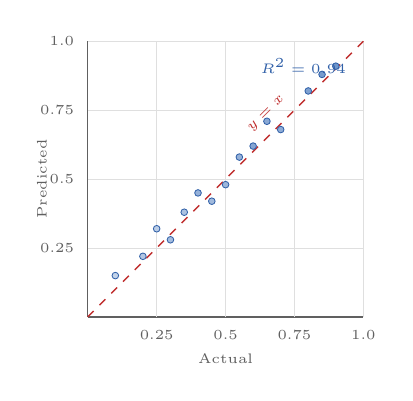
\begin{tikzpicture}

%% COPY-START =========================================================

% --- DATA (replace with your actual data points) ---
% Each entry: actual_x / predicted_y / color_intensity (0-100)
\def\scatdata{%
  0.1/0.15/40, 0.2/0.22/50, 0.3/0.28/60,
  0.4/0.45/70, 0.5/0.48/65, 0.6/0.62/80,
  0.7/0.68/75, 0.8/0.82/85, 0.85/0.88/90,
  0.9/0.91/95, 0.25/0.32/45, 0.55/0.58/70,
  0.65/0.71/78, 0.45/0.42/62, 0.35/0.38/55%
}
\def\xO{0}
\def\yO{0}
\def\chartW{3.5}        % plot width in cm
\def\chartH{3.5}        % plot height in cm
\def\xMax{1.0}
\def\yMax{1.0}

% --- AXES ---
\draw[acaGreyLine, line width=0.5pt]
  (\xO, \yO) -- (\xO + \chartW, \yO);
\draw[acaGreyLine, line width=0.5pt]
  (\xO, \yO) -- (\xO, \yO + \chartH);

% --- GRIDLINES (every 0.25) ---
\foreach \t in {0.25, 0.5, 0.75, 1.0} {
  \pgfmathsetmacro\xt{\xO + \chartW * \t / \xMax}
  \pgfmathsetmacro\yt{\yO + \chartH * \t / \yMax}
  % vertical gridline
  \draw[acaGreyLine!20, line width=0.2pt]
    (\xt, \yO) -- (\xt, \yO + \chartH);
  % horizontal gridline
  \draw[acaGreyLine!20, line width=0.2pt]
    (\xO, \yt) -- (\xO + \chartW, \yt);
  % tick labels
  \node[font=\tiny, color=acaGreyLine, anchor=north]
    at (\xt, \yO - 0.05) {\t};
  \node[font=\tiny, color=acaGreyLine, anchor=east]
    at (\xO - 0.05, \yt) {\t};
}

% --- DIAGONAL REFERENCE LINE (y = x) ---
\draw[acaRedLine, dashed, line width=0.5pt]
  (\xO, \yO) -- (\xO + \chartW, \yO + \chartH);
\node[font=\tiny, color=acaRedLine, anchor=south west, rotate=45]
  at ($(\xO + \chartW*0.6, \yO + \chartH*0.6) + (0, 0.05)$)
  {$y = x$};

% --- SCATTER POINTS ---
\foreach \xv/\yv/\c in \scatdata {
  \pgfmathsetmacro\px{\xO + \chartW * \xv / \xMax}
  \pgfmathsetmacro\py{\yO + \chartH * \yv / \yMax}
  \fill[acaBlueFill!\c!white, draw=acaBlueLine, line width=0.3pt]
    (\px, \py) circle (1.2pt);
}

% --- AXIS LABELS ---
\node[font=\tiny, color=acaGreyLine, anchor=north]
  at (\xO + \chartW/2, \yO - 0.35) {Actual};
\node[font=\tiny, color=acaGreyLine, anchor=south, rotate=90]
  at (\xO - 0.4, \yO + \chartH/2) {Predicted};

% --- R^2 ANNOTATION (right corner) ---
\node[font=\tiny, color=acaBlueLine, anchor=north east]
  at (\xO + \chartW - 0.1, \yO + \chartH - 0.1) {$R^2 = 0.94$};

%% COPY-END ===========================================================

\end{tikzpicture}
\end{document}
